\chapter{Introduction to Common Intermediate Language}
\section{CIL Fundamentals}
The way CIL code get written are arranged by stack. So assume we have the following code in C\#:
\lstinputlisting[style=customcs]{codes/Chap7/Chap7Snippet1.cs}
That code would be compiled as follow:
\lstinputlisting[style=customcs]{codes/Chap7/Chap7Snippet2.cs}

There are few things happening here:
The shorthand CIL opcode, "ldarg.0", loads the first parameter, int a, to the stack. "ldarg.0" is a short hand opcode that you do not have to specify an argument for which parameter to load after opcode, so it save space and serves as a shortcut for runtime to infers what operation to build for that opcode.

Then "ldarg.1" do a similar operation to the above, but load the second parameter onto the stack. The "add" operation requires no arguments, but it pop off 2 items off the stack, so in "add" opcode point of view, when it pop the stack, it would see "ldarg.1" first and then "ldarg.0" second, this is something to keep in mind if you were to plan on writing a new runtime. The "add" opcode will arrange the items that were popped off the stack and do an addition operation from there (it uses the left-hand value type for addition) and then push the result of the addition to the stack.

Now that we have one remaining item in our stack, the "ret" opcode will pop the item off the stack and return that value for function return value.
\newpage
In an effort to help you actually be able to visualize and understand how this works:

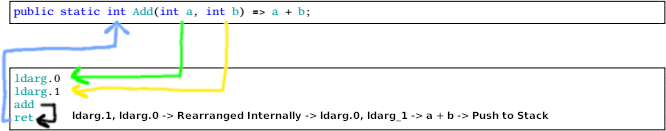
\includegraphics[width=\textwidth]{ChapSevenVisual}

\section{Special Note about the Stack}
\textit{Note: This is a simple warning for those who use Stack in .Net Framework.}

Stack is a Last In First Out, LIFO, so basically the last item you \textbf{push} to the stack is going to be the first item you get when you \textbf{pop} the stack. In .Net Framework, when you attempt to use the IEnumerator of Stack<T>, it will use the pop order in the way you read, so if you for an example have the following code:

\lstinputlisting[style=customcs]{codes/Chap7/Chap7Snippet3.cs}

There is a few things happening here, the stack would be reversed when the following code get called:

\lstinputlisting[style=customcs]{codes/Chap7/Chap7Snippet5.cs}

The stack already get reversed, because remember, the IEnumerator in Stack<T> is read by pop order, so when you pop and push to alternative stack, it rearrange the items like so:

ABC -> CBA -> ABC

To avoid this, you simply just have the following code instead of having to do any additional operations:

\lstinputlisting[style=customcs]{codes/Chap7/Chap7Snippet4.cs}
